% !TEX root = /Users/zhuzhuangdi/Desktop/MSUCourses/NaturalLanguageProcessing842/Project/Proposal/main.tex
\section{Evaluation}
We plan to complete our project in the following five steps:


\begin{itemize}
\item {Background Survey and Corpus Collection.}  
%
For survey, we will look at the following specific aspects: vector space representation, semantic compositionality, neural-network models, and bag-of-words models.
%
Better understanding of related work will provide us with great help for the following work, especially on model implementation and comparison. 
%
For corpus collection, we will use the dataset mentioned in Section \ref{subsec:data} for training/testing our model.
\item {Model Implementation.}
Second, implementation of the recursive model would be the most important work in our project. 
%
So we will assign more time on this step.  We will use Stanford's open-source code for parse tree generations, and also use their MV-RNN model to start with our project.

\item {Model Testing and Optimization.} 
%
Third, we will compare the performance of our model with existing approachesl.
%
In this step, we will continue to tune our model, and explore more features to improve  model performance, such as micro-blog features including emotions and hashtags.
%
The metric for our model evaluation would be  F-measure and cross-validation accuracy.

\item {Project Summary and Writing} We will start to record experiment data when we are at the model testing step. Finally we will spend around one week to organize our discovery and finish our project report.
\end{itemize}

Below is a visualization of our project timeline:
\begin{figure}[htbp]
	\centering
	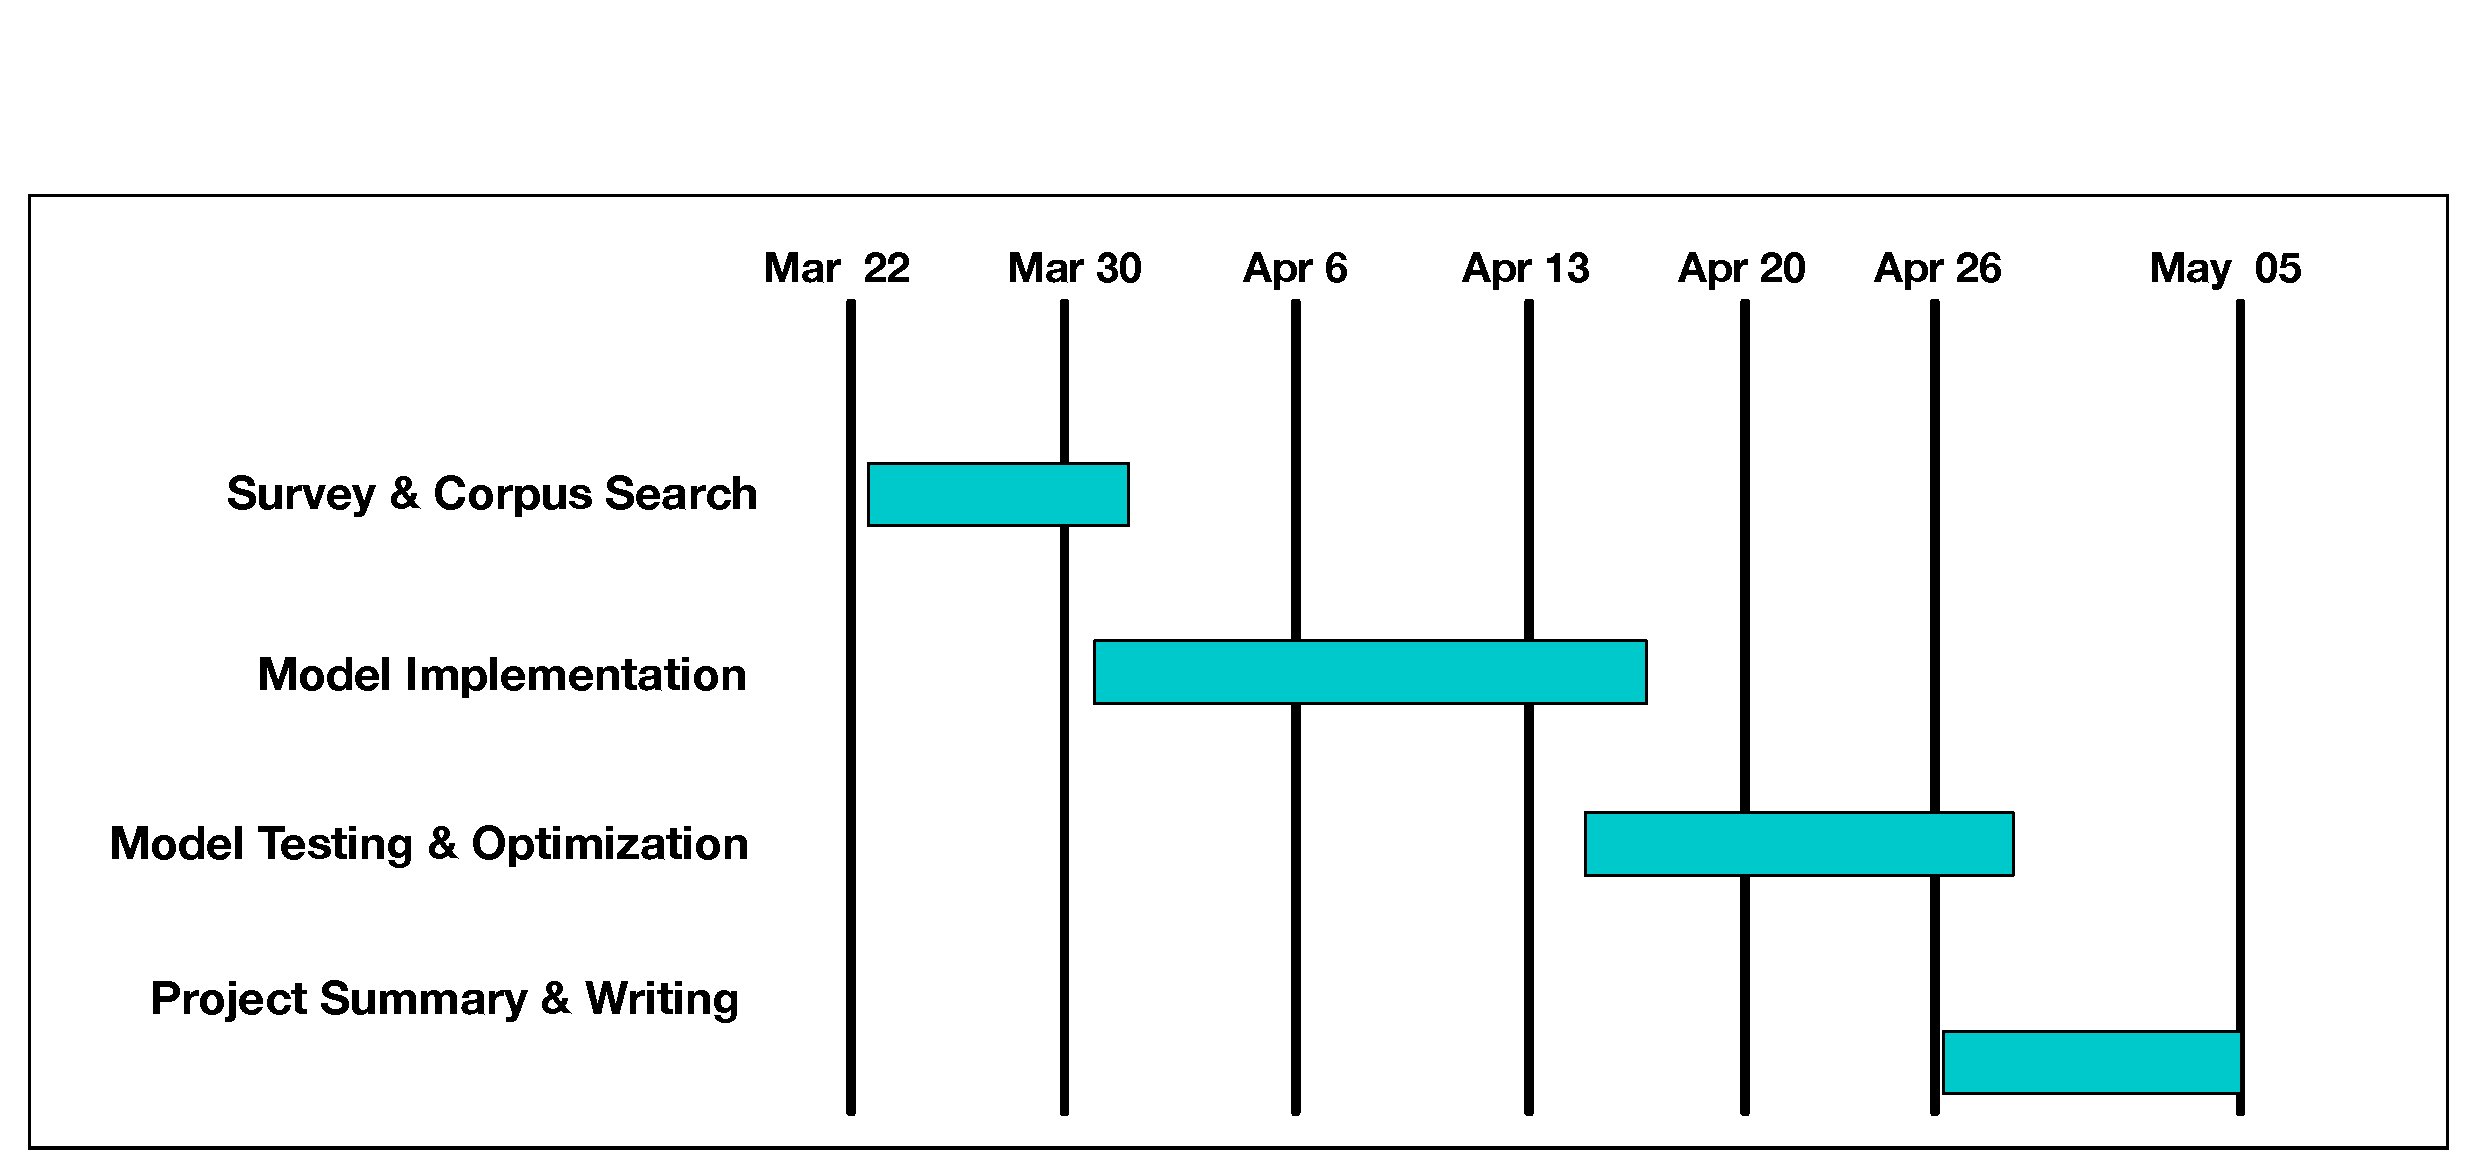
\includegraphics[width=1.1\linewidth]{mileStone}
	\caption{Project Timeline}
	\label{fig:projecttimeline}	
\end{figure}
 

